\documentclass{article}\usepackage[]{graphicx}\usepackage[]{color}
% maxwidth is the original width if it is less than linewidth
% otherwise use linewidth (to make sure the graphics do not exceed the margin)
\makeatletter
\def\maxwidth{ %
  \ifdim\Gin@nat@width>\linewidth
    \linewidth
  \else
    \Gin@nat@width
  \fi
}
\makeatother

\definecolor{fgcolor}{rgb}{0.345, 0.345, 0.345}
\newcommand{\hlnum}[1]{\textcolor[rgb]{0.686,0.059,0.569}{#1}}%
\newcommand{\hlstr}[1]{\textcolor[rgb]{0.192,0.494,0.8}{#1}}%
\newcommand{\hlcom}[1]{\textcolor[rgb]{0.678,0.584,0.686}{\textit{#1}}}%
\newcommand{\hlopt}[1]{\textcolor[rgb]{0,0,0}{#1}}%
\newcommand{\hlstd}[1]{\textcolor[rgb]{0.345,0.345,0.345}{#1}}%
\newcommand{\hlkwa}[1]{\textcolor[rgb]{0.161,0.373,0.58}{\textbf{#1}}}%
\newcommand{\hlkwb}[1]{\textcolor[rgb]{0.69,0.353,0.396}{#1}}%
\newcommand{\hlkwc}[1]{\textcolor[rgb]{0.333,0.667,0.333}{#1}}%
\newcommand{\hlkwd}[1]{\textcolor[rgb]{0.737,0.353,0.396}{\textbf{#1}}}%
\let\hlipl\hlkwb

\usepackage{framed}
\makeatletter
\newenvironment{kframe}{%
 \def\at@end@of@kframe{}%
 \ifinner\ifhmode%
  \def\at@end@of@kframe{\end{minipage}}%
  \begin{minipage}{\columnwidth}%
 \fi\fi%
 \def\FrameCommand##1{\hskip\@totalleftmargin \hskip-\fboxsep
 \colorbox{shadecolor}{##1}\hskip-\fboxsep
     % There is no \\@totalrightmargin, so:
     \hskip-\linewidth \hskip-\@totalleftmargin \hskip\columnwidth}%
 \MakeFramed {\advance\hsize-\width
   \@totalleftmargin\z@ \linewidth\hsize
   \@setminipage}}%
 {\par\unskip\endMakeFramed%
 \at@end@of@kframe}
\makeatother

\definecolor{shadecolor}{rgb}{.97, .97, .97}
\definecolor{messagecolor}{rgb}{0, 0, 0}
\definecolor{warningcolor}{rgb}{1, 0, 1}
\definecolor{errorcolor}{rgb}{1, 0, 0}
\newenvironment{knitrout}{}{} % an empty environment to be redefined in TeX

\usepackage{alltt}

\usepackage{hyperref}

\hypersetup{
    colorlinks=true,
    linkcolor=blue,
    filecolor=magenta,      
    urlcolor=cyan,
}

\usepackage{listings}
\usepackage{color}

\definecolor{dkgreen}{rgb}{0,0.6,0}
\definecolor{gray}{rgb}{0.5,0.5,0.5}
\definecolor{mauve}{rgb}{0.58,0,0.82}

\lstset{frame=tb,
  language=bash,
  aboveskip=3mm,
  belowskip=3mm,
  showstringspaces=false,
  columns=flexible,
  basicstyle={\small\ttfamily},
  numbers=none,
  numberstyle=\tiny\color{gray},
  keywordstyle=\color{blue},
  commentstyle=\color{dkgreen},
  stringstyle=\color{mauve},
  breaklines=true,
  breakatwhitespace=true,
  tabsize=3
}

\author{Anna Burns}
\title{Precipitation and Peak Stream Flows of the Des Plaines River, Northern IL}
\IfFileExists{upquote.sty}{\usepackage{upquote}}{}
\begin{document}
\maketitle

\section*{Introduction}

  Northern Illinois is a prairie-forest glaciated landscape with a historically high-organic-content loess soil that has been eroded by extensive industrial agriculture over the past 150 years to a clay-dense soil B-horizon (Knox).  The region is populated largely by towns with populations under 30,000 who work both in local industry and in commuting to Chicago or Milwaukee.  Agriculture is also common in the area, with large fields of cash crops such as corn and soy as well as smaller produce farms.  Calculated for the 1981-2010 climate normals, the Antioch Illinois Weather Service Station reports that the mean January temperature is 21.9 degF, with an average of 28.5 days below 32 degrees and 5.5 days below 0 degrees (without accounting for windchill).  In contrast, the average July temperature is 73.5 degF, with an average of 3.5 days above 90 degF.  The annual mean precipitation for the region is 36.7 inches (the majority of which tends to fall in the summer months), with an annual mean snowfall of 42.7 inches.  

Precipitation presents an interesting challenge under both climate change and land use change events. Precipitation data obtained from the National Oceanic and Atmospheric Association's (NOAA) Climate Data Online regarding the Antioch weather station reveals lack of general precipitation trends between 1901 and 2008 (with a gap in the data between 1922 and 1941).  In contrast, the U.S. Geological Survey's National Water Information System Des Plaines River metering station in Russell, IL (approximately ten miles from Antioch) displays significant trends in streamflow levels during peak flow events from 1960 to 2019.  This data is collected in coordination of Illinois Department of Natural Resources' Office of Water Resources, near the Illinois-Wisconsin border and the Sterling Lake system.  The river narrows significantly a few miles past Russell in the Wisconsin portion of the watershed, but is at a representative width for the Lake County Des Plaines River watershed by the time it reaches the meter station in Russell, IL.

The increase in streamflow during annual peak flow events without a corresponding trend in increasing mean annual precipitation is concerning.  This trend provides support for NOAA's finding that there has been a state-wide increase in number and severity of extreme precipitation events (Frankson and Kunkel, 2017).  Increases in these events combined with the changes in soil described by Knox (2001) from a organically-rich loess to a clay-dense soil due to agricultural land use, as well as increases in nonpermeable surfaces with increased urbanization of the area, put more stress on the watershed to accomodate increased water levels during precipitation events.  These changes are detailed in Frans et. al (2013), which conducted a hydrologic model study of the Upper Mississippi River Valley (including northern Illinois) to determine that in spite of land use changes, upwards of 90 percent of changes in water runoff in the region were due to climate change-driven factors.  This suggests that as Illinois feels the impacts of climate change described Cherkauer and Sinha (2010) -- which includes increasing in spring rain and a 22-31\% increase in high stream flow days -- that northern Illinois region will become increasingly susceptible to flooding events.

This paper examines streamflow volume of the Des Plaines River during peak flow events between 1967 and 2019.  The increased levels of stream flow reflect both changes in permeable surfaces and historic changes in soil composition due to agriculture industry; although there is no evidence to suggest an increase in precipitation over the period studied, predictions for the impact of climate change on the region through the 21st century suggest that that these factors will increasingly impact peak stream flow levels.
  
\section*{Data Analysis}

After obtaining the data from daily precipitation data (in cm) from NOAA's CDO database, the sum of the precipitation levels were aggregated for each month between 1901 and 2008, excluding the missing data between 1922 and 1941.  Then, the sum of the monthly precipitation was graphed over time for each of the twelve months, and a linear model was applied to each month's precipitation trend using a 5\% confidence level under the null hypothesis that there is no correlation between monthly precipitation sums and time.  The results of this linear regression are broken down by month in Table 1, and display low levels of correlation over time.  None of the months demonstrate a significant correlation between monthly precipitation sums and time, and the null hypothesis stands.

\emph{Table 1. Antioch, IL Monthly Precipitation Trends (1901 to 2008)}
\begin{table}[ht]
\centering
\begin{tabular}{rllll}
  \hline
 & Month & Slope & P & R-Sq \\ 
  \hline
  & January & -0.0286 & 0.754 & 0.001 \\ 
  & February & 0.0108 & 0.8872 & 0 \\ 
  & March & -0.1121 & 0.358 & 0.01 \\ 
  & April & 0.0301 & 0.8318 & 0.001 \\ 
  & May & -0.0416 & 0.8024 & 0.001 \\ 
  & June & 0.2584 & 0.1491 & 0.025 \\ 
  & July & 0.0785 & 0.6443 & 0.003 \\ 
  & August & 0.3523 & 0.0565 & 0.042 \\ 
  & September & -0.1826 & 0.4162 & 0.008 \\ 
  & October & -0.0296 & 0.8485 & 0 \\ 
  & November & 0.2177 & 0.0587 & 0.042 \\ 
  & December & 0.0918 & 0.3863 & 0.009 \\ 
   \hline
\end{tabular}
\end{table}
\newpage

Next, data regarding streamflow levels during peak flow events on the Des Plaines River were obtained from the U.S. Geological Survey's site at Russell, IL, located approximately ten miles from Antioch.  This data contains the streamflow (cubic feet per second) and discharge levels (feet) during the peak annual streamflow events for every year between 1960 and 2019.  The streamflow levels was plotted against time, and a linear regression model was applied to the data.  Once again, this linear regression operated at a 5\% confidence level, with the null hypothesis that streamflow during peak flow events had not changed over time.  A BoxCox graph revealed that the data would benefit from a logarithmic adjustment to correct for variation in the data, and this transformation was applied.  The best fit line and plotted data is included in Graph 1.

\begin{knitrout}
\definecolor{shadecolor}{rgb}{0.969, 0.969, 0.969}\color{fgcolor}
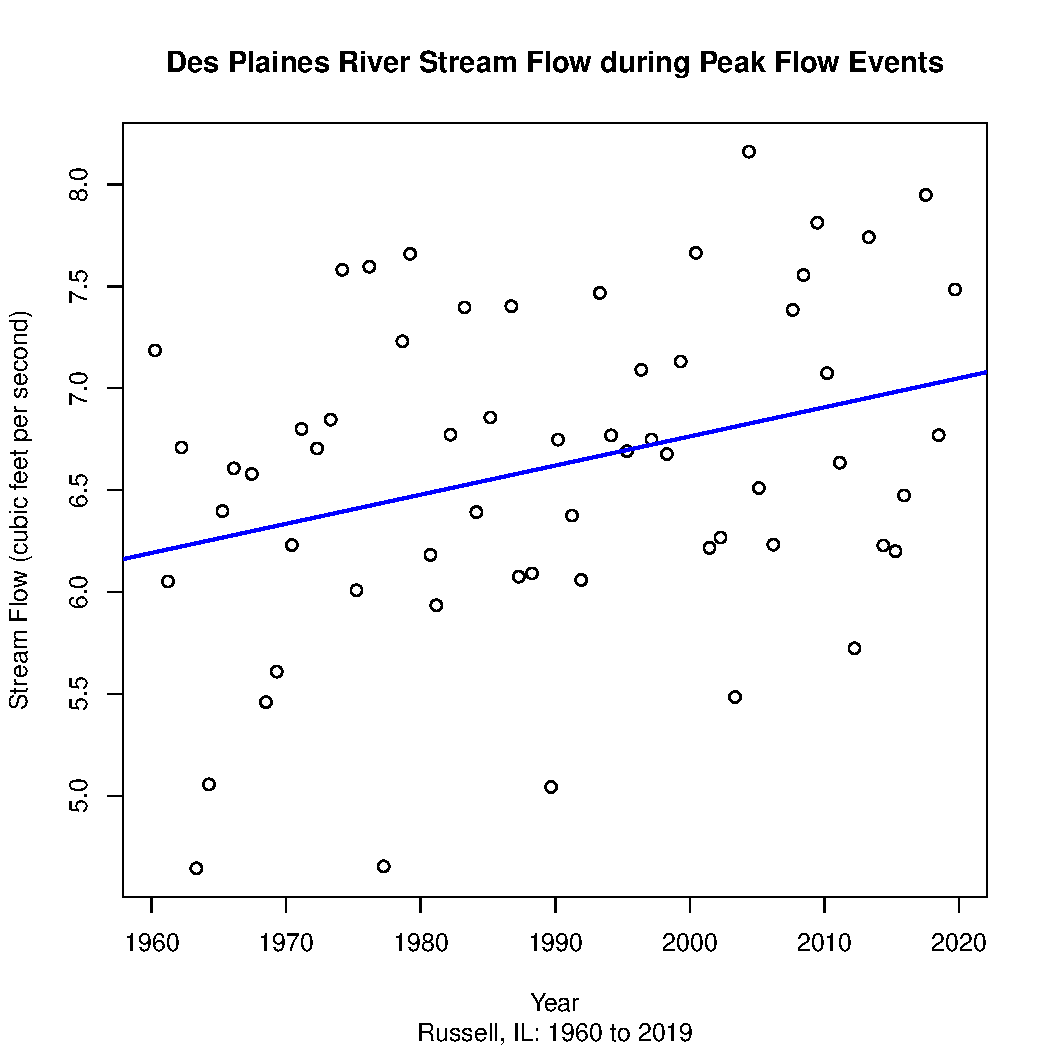
\includegraphics[width=\maxwidth]{figure/unnamed-chunk-1-1} 

\end{knitrout}

The linear regression had a p-value of 0.016, meaning that the null hypothesis that there was no correlation between peak streamflow levels and time could be comfortably rejected.  There is evidence to suggest that streamflow levels during peak flow events have increased between 1960 and 2019.  Although the correlation is low with an adjusted R-squared of 0.1 (meaning that approximately 10 percent of the variation in peak annual stream flow levels can be explained by the variation in the date), because natural phenomenon have so many conflicting variables this level of correlation is satisfactory.  Although the data fails the independence assumption for linear modeling (because the datapoints fall on sequential dates), once a logarithmic transformation was applied the data was sufficiently homoskedastic, normal, and linear for the model to still be used.  

\section*{Conclusions}

These results have a significant impact on the Des Plaines Watershed, demonstrating the vulnerability of the system to extreme precipitation events.  As discussed in Cherkauer and Sinha (2010), increase in extreme precipitation events is one of the greatest impacts of climate change on Illinois.  The sensitivity of the Des Plaines River Watershed to these events will leave Lake County communities vulnerable to flooding as the 21st century continues.

Skeptics may question the validity of this assertion on two grounds: that northern Illinois is not expected to see an immediate increase in precipitation levels, and that precipitation levels have not been shown to increase in the region over the past century in spite of rising global temperatures.  However, this data does not describe overall levels in precipitation, but rather extreme precipitation events. Cherkauer and Sinha (2010) describe that while precipitation levels may not increase immediately in northern Illinois, the bulk of the rainfall will likely shift from the summer to the spring.  Furthermore, this rainfall is more likely to be condensed into extreme precipitation events, which will have more of a damaging imapct on the Des Plaines watershed than rain events over a long period of time would.  

This data directly reflects Cherkauer and Sinha's analysis that peak stream flow events will become more severe across the Upper Mississippi River Valley.  Although this is partially a reflection of the land use change described by Knox (2001), it is likely further impacted by global climate change as detailed in Frans et al. (2013).  

This data suggests that Lake County communities along the Des Plaines River could be highly impacted by the sensitivity of the watershed to extreme precipitation events.  Outdated infrastructure, including combined stormwater-sewage systems, could be overwhelmed by increased water levels, increasing instances of waterborne illnesses (Patz, 2014).  Additionally, agriculture could be negatively impacted by extreme rainfall events as crops are damaged by precipitation, or because water availability will be lower during the summer as precipitation falls more heavily in the spring (Hatfield 2014).  This implicates severe human health and economic impacts of climate change on the northern Illinois region.  Some of these impacts can be mitigated by updating infrastructure and informing citizens about protecting their homes from flooding.  However, to fully stem the impacts of climate change on northern Illinois, a transformation of the economy's reliance on fossil fuels will be necessary in order to stem the worst effects of global climate change on northern Illinois' most vulnerable citizens.

\section*{Works Cited}

\begin{itemize}
  \item Angel, J. (2020).  "Official 1981-2010 Climate Normals." Illinois State Water Survey.  Accessed 25 September, 2020 from https://www.isws.illinois.edu/statecli/newnormals/normals.USC00110203.txt. 
  \item Cherkauer, K.A. \& Sinha, T. (2010). “Hydrologic impacts of projected future climate change in 	the Lake Michigan region.”  Journal of Great Lakes Research, 36, pp. 33-50.  DOI: 	10.1016/j.jglr.2009.11.012.
  \item Frankson, R., K. Kunkel, S. Champion, B. Stewart, D. Easterling, B. Hall, and J. R. Angel. (2017). "Illinois State Climate Summary." NOAA Technical Report NESDIS 149-IL (4).
  \item Frans, C., et al. (2013).  “Are climactic or land cover changes the dominant cause of runoff 	trends in the Upper Mississippi River Basin?” Geophysical Research Letters, 40, pp. 	1104-1110.  DOI: 10.1002/grl.50262. 
  \item Hatfield, J.L. (2014).  “Agriculture in the Midwest.”  In J.A. Winkler, et al. (Eds.), Climate 	change in the Midwest: A synthesis report for the National Climate Assessment, pp. 188-	196.  Island Press.
  \item Knox, J.C. (2001).  “Agricultural influence on landscape sensitivity in the Upper Mississippi 	River Valley.”  Catena, 42(2-4), pp. 193-224.  DOI: 10.1016/S0341-8162(00)00138-7.
  \item Patz, J. (2014).  “Health.”  In J.A. Winkler, et al. (Eds.), Climate change in the Midwest: A 	synthesis report for the National Climate Assessment, pp. 188-196.  Island Press.
\end{itemize}

\end{document}
